% This template was minimally adapted from Steven V. Miller's template for academic manuscripts. See:
% http://svmiller.com/blog/2016/02/svm-r-markdown-manuscript/
\documentclass[]{article}
\usepackage[left=1in,top=1in,right=1in,bottom=1in]{geometry}
\newcommand*{\authorfont}{\fontfamily{phv}\selectfont}
\usepackage{lmodern}


\usepackage[T1]{fontenc}
\usepackage[utf8]{inputenc}


\usepackage{abstract}
\renewcommand{\abstractname}{}    % clear the title
\renewcommand{\absnamepos}{empty} % originally center

\renewenvironment{abstract}
 {{%
    \setlength{\leftmargin}{0mm}
    \setlength{\rightmargin}{\leftmargin}%
  }%
  \relax}
 {\endlist}

\makeatletter
\def\@maketitle{%
  \newpage
%  \null
%  \vskip 2em%
%  \begin{center}%
  \let \footnote \thanks
    {\fontsize{18}{20}\selectfont\raggedright  \setlength{\parindent}{0pt} \@title \par}%
}
%\fi
\makeatother




\setcounter{secnumdepth}{0}


\usepackage{graphicx,grffile}
\makeatletter
\def\maxwidth{\ifdim\Gin@nat@width>\linewidth\linewidth\else\Gin@nat@width\fi}
\def\maxheight{\ifdim\Gin@nat@height>\textheight\textheight\else\Gin@nat@height\fi}
\makeatother
% Scale images if necessary, so that they will not overflow the page
% margins by default, and it is still possible to overwrite the defaults
% using explicit options in \includegraphics[width, height, ...]{}
\setkeys{Gin}{width=\maxwidth,height=\maxheight,keepaspectratio}


\title{The Relationship between Urban Green Space and Socioeconomic
Factors in the City of Vancouver: A Case of Environmental
Injustice \thanks{Paper submitted to complete the requirements of
ENVSOCTY 4GA3 Applied Spatial Statistics; with additional edits by
Antonio Paez for this version.}  }
 



\author{\Large Daina De
Angelis\vspace{0.05in} \newline\normalsize\emph{400240413}   \and \Large Tim
Truong\vspace{0.05in} \newline\normalsize\emph{400264793}   \and \Large Maeve
Nowitsky\vspace{0.05in} \newline\normalsize\emph{400264259}   \and \Large Jillian
Mezenberg\vspace{0.05in} \newline\normalsize\emph{400243427}  }


\date{}

\usepackage{titlesec}

\titleformat*{\section}{\normalsize\bfseries}
\titleformat*{\subsection}{\normalsize\itshape}
\titleformat*{\subsubsection}{\normalsize\itshape}
\titleformat*{\paragraph}{\normalsize\itshape}
\titleformat*{\subparagraph}{\normalsize\itshape}





\newtheorem{hypothesis}{Hypothesis}
\usepackage{setspace}


% set default figure placement to htbp
\makeatletter
\def\fps@figure{htbp}
\makeatother

\usepackage{fvextra} \DefineVerbatimEnvironment{Highlighting}{Verbatim}{breaklines,commandchars=\\\{\}}
\usepackage{booktabs}
\usepackage{longtable}
\usepackage{array}
\usepackage{multirow}
\usepackage{wrapfig}
\usepackage{float}
\usepackage{colortbl}
\usepackage{pdflscape}
\usepackage{tabu}
\usepackage{threeparttable}
\usepackage{threeparttablex}
\usepackage[normalem]{ulem}
\usepackage{makecell}
\usepackage{xcolor}

% move the hyperref stuff down here, after header-includes, to allow for - \usepackage{hyperref}

\makeatletter
\@ifpackageloaded{hyperref}{}{%
\ifxetex
  \PassOptionsToPackage{hyphens}{url}\usepackage[setpagesize=false, % page size defined by xetex
              unicode=false, % unicode breaks when used with xetex
              xetex]{hyperref}
\else
  \PassOptionsToPackage{hyphens}{url}\usepackage[draft,unicode=true]{hyperref}
\fi
}

\@ifpackageloaded{color}{
    \PassOptionsToPackage{usenames,dvipsnames}{color}
}{%
    \usepackage[usenames,dvipsnames]{color}
}
\makeatother
\hypersetup{breaklinks=true,
            bookmarks=true,
            pdfauthor={Daina De Angelis (400240413) and Tim
Truong (400264793) and Maeve Nowitsky (400264259) and Jillian
Mezenberg (400243427)},
             pdfkeywords = {},  
            pdftitle={The Relationship between Urban Green Space and
Socioeconomic Factors in the City of Vancouver: A Case of Environmental
Injustice},
            colorlinks=true,
            citecolor=blue,
            urlcolor=blue,
            linkcolor=magenta,
            pdfborder={0 0 0}}
\urlstyle{same}  % don't use monospace font for urls

% Add an option for endnotes. -----


% add tightlist ----------
\providecommand{\tightlist}{%
\setlength{\itemsep}{0pt}\setlength{\parskip}{0pt}}

% add some other packages ----------

% \usepackage{multicol}
% This should regulate where figures float
% See: https://tex.stackexchange.com/questions/2275/keeping-tables-figures-close-to-where-they-are-mentioned
\usepackage[section]{placeins}


\begin{document}
	
% \pagenumbering{arabic}% resets `page` counter to 1 
%    

% \maketitle

{% \usefont{T1}{pnc}{m}{n}
\setlength{\parindent}{0pt}
\thispagestyle{plain}
{\fontsize{18}{20}\selectfont\raggedright 
\maketitle  % title \par  

}

{
   \vskip 13.5pt\relax \normalsize\fontsize{11}{12} 
\textbf{\authorfont Daina De
Angelis} \hskip 15pt \emph{\small 400240413}   \par \textbf{\authorfont Tim
Truong} \hskip 15pt \emph{\small 400264793}   \par \textbf{\authorfont Maeve
Nowitsky} \hskip 15pt \emph{\small 400264259}   \par \textbf{\authorfont Jillian
Mezenberg} \hskip 15pt \emph{\small 400243427}   

}

}






\vskip -8.5pt


 % removetitleabstract

\noindent  

\hypertarget{r-markdown}{%
\subsection{R Markdown}\label{r-markdown}}

This is an R Markdown document. Markdown is a simple formatting syntax
for authoring HTML, PDF, and MS Word documents. For more details on
using R Markdown see \url{http://rmarkdown.rstudio.com}.

When you click the \textbf{Knit} button a document will be generated
that includes both content as well as the output of any embedded R code
chunks within the document. You can embed an R code chunk like this:

Note that the \texttt{echo\ =\ FALSE} parameter was added to the code
chunk to prevent printing of the R code that generated the plot.

\#Introduction

\#Background

\#Study Area

This study took place at the Census Subdivision level to target the
municipality of Vancouver, BC. There are 127 census tracts in Vancouver
that were studied.

\#Data

\begin{verbatim}
The data used for analysis includes census data for variables of population, population density, visible minority status, non-visible minority status, and income for each census tract in the census subdivision of Vancouver. This data was obtained from Statistics Canada through use of the cancensus package in R. All census data used is from the 2021 census. Point data for each the location of each park, homeless shelter, and street tree in the census subdivision was downloaded in a .csv file format from the City of Vancouver’s open data portal. To use the r5r package so that accessibility to parks by both walking and public transit could be determined, a road network dataset of Vancouver, and as well as a public transport feed of the city was needed. The road network dataset was obtained from BBBike, and was stored as a .pbf file. The public transport feed was obtained from Transitland and stored in a GTFS.zip file. 
\end{verbatim}

\#Methods

\begin{verbatim}
To determine the relationship between greenspace and other socioeconomic factors in Vancouver, Rstudio was used to analyze and visualize the variables being examined. Choropleth maps for variables of population, population density, visible minority status, non-visible minority status, and income, and accessibility to parks were made to provide a visual representation of the difference between census tracts. Regression analysis was used to determine the relationship between the independent variable studied (number of parks accessible within a 30 minute travel time) and dependent variables (population, population density, visible minority status, non-visible minority status, and income). Scatterplots were used to show a visual representation between independent and dependent variables studied to better understand the results of regression analysis. 
\end{verbatim}

\#Results

\begin{verbatim}
To begin our analysis, the centroids for each census tract in the Vancouver CSD were obtained and put into a dataframe with latitude, longitude, and census ID. This allowed us to have point data describing the middle of each CT.
\end{verbatim}

The point data for park in the Vancouver CSD was obtained from a csv
file from Vancouver's open data portal and transformed into a data frame
with columns describing the X and Y coordinates of each park.

The point data for parks was prepared for use of the r5r package by
renaming coulumns for latitude, longitude, and park ID data and to the
names required by r5r. Data for latitude and longitude was converted
into a numeric format. Lastly, a column to indicate that each park point
was one singular park was added to meet the requirement of the
opportunites parameter in r5r.

Next, the r5r package was used in order to build a transport network for
Vancouver, so that the distances and routing between the centroids of
census tracts and park locations can be calculated.

The transport network was built with using a road network dataset of
Vancouver, and as well as a public transport feed of the city. The road
network dataset was obtained from BBBike, and was stored as a .pbf file.
The public transport feed was obtained from Transitland and stored in a
GTFS.zip file.

The accessibility function in r5r was used to compute how many parks
were accessible within 30 minutes of each census tracts centroid by
walking or public transit.

Once the number of accessible parks was calculated, this was added to
the data frame displaying census data.

After all variables were in one data frame and prepared for analysis,
data was first visualized by creating choropleth maps for each variable
of interest. Maps were created for each variable as follows:

Population of each CT

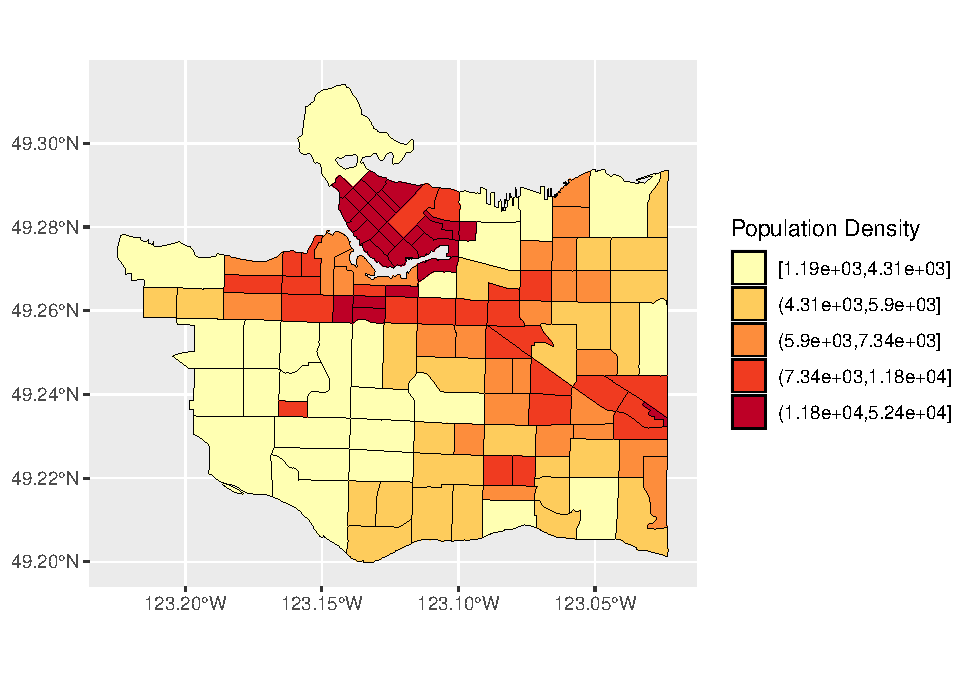
\includegraphics{4GA3Markdown_files/figure-latex/unnamed-chunk-23-1.pdf}

Population density of each CT

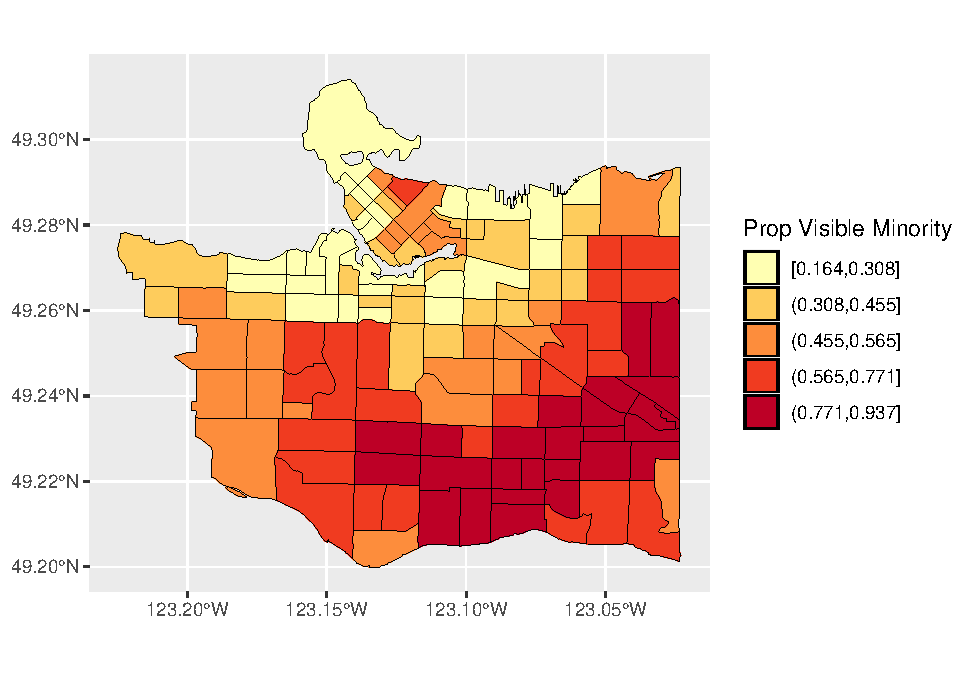
\includegraphics{4GA3Markdown_files/figure-latex/unnamed-chunk-24-1.pdf}
Proportion of population identifying as visible and non-visible
minorities

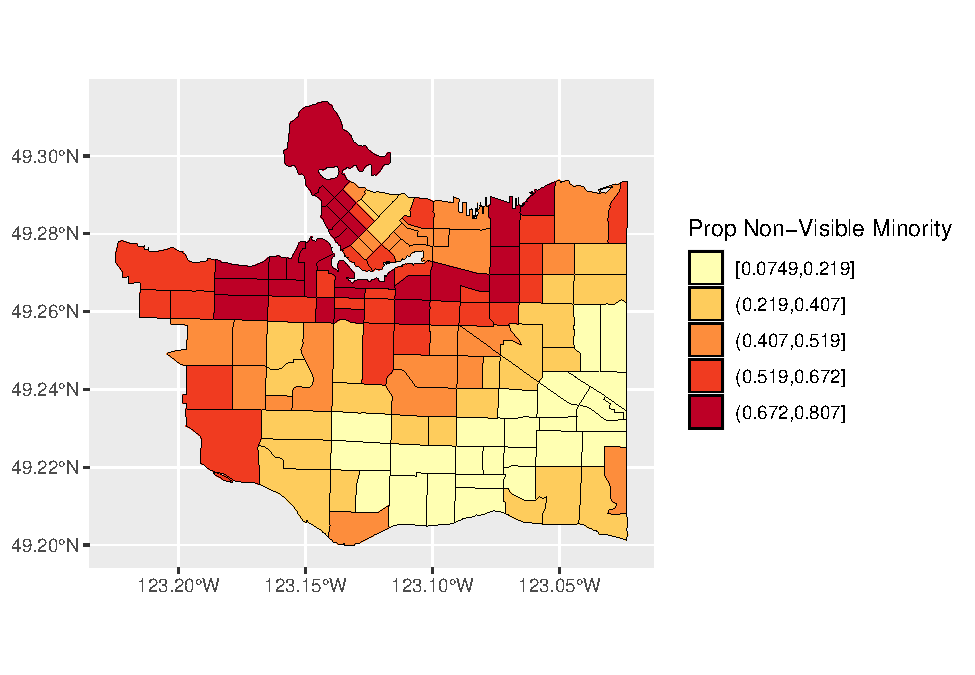
\includegraphics{4GA3Markdown_files/figure-latex/unnamed-chunk-25-1.pdf}

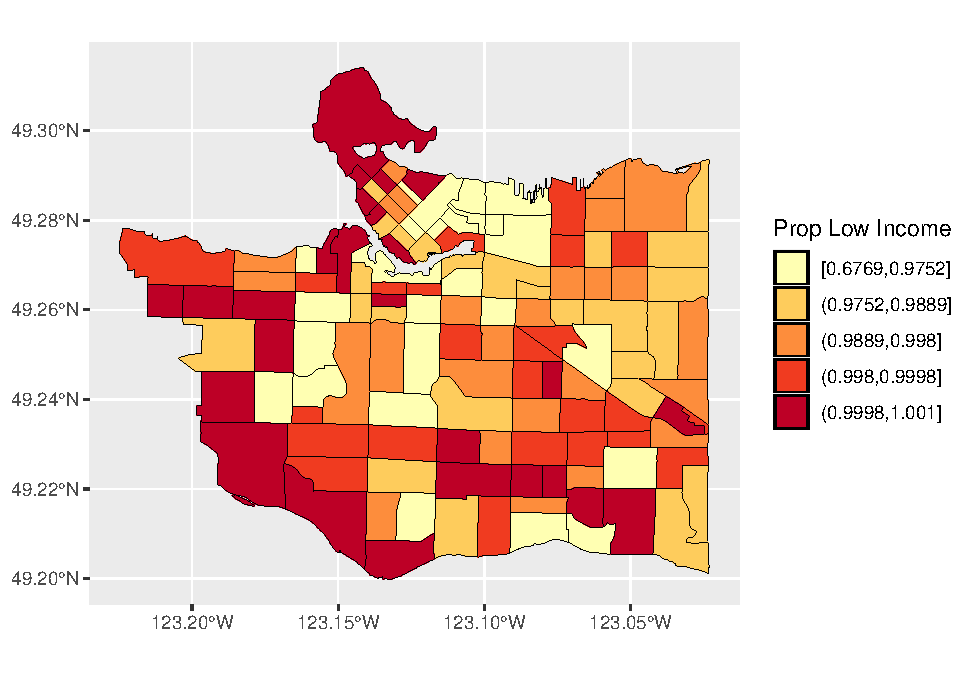
\includegraphics{4GA3Markdown_files/figure-latex/unnamed-chunk-26-1.pdf}

The proportion of the population considered low income for each CT

\includegraphics{4GA3Markdown_files/figure-latex/unnamed-chunk-27-1.pdf}

Finally, a choropleth map was created to display the independent
variable, parks accessible within 30 minutes of a centroid.

\includegraphics{4GA3Markdown_files/figure-latex/unnamed-chunk-28-1.pdf}

Next, to determine the relationship between the number of accessible
parks and each independent variable, the independent variables were
regressed to number of accessible parks for each CT.

\begin{table}[!htbp] \centering 
  \caption{Population of Census Tracts regressed on Number of Parks Accessible} 
  \label{} 
\begin{tabular}{@{\extracolsep{5pt}}lc} 
\\[-1.8ex]\hline 
\hline \\[-1.8ex] 
 & \multicolumn{1}{c}{\textit{Dependent variable:}} \\ 
\cline{2-2} 
\\[-1.8ex] & Population\_2021 \\ 
\hline \\[-1.8ex] 
 accessibility & 10.518 \\ 
  & (7.816) \\ 
  & \\ 
 Constant & 4,904.639$^{***}$ \\ 
  & (264.208) \\ 
  & \\ 
\hline \\[-1.8ex] 
Observations & 127 \\ 
R$^{2}$ & 0.014 \\ 
Adjusted R$^{2}$ & 0.006 \\ 
Residual Std. Error & 1,459.451 (df = 125) \\ 
F Statistic & 1.811 (df = 1; 125) \\ 
\hline 
\hline \\[-1.8ex] 
\textit{Note:}  & \multicolumn{1}{r}{$^{*}$p$<$0.1; $^{**}$p$<$0.05; $^{***}$p$<$0.01} \\ 
\end{tabular} 
\end{table}

For each regression, a scatter plot was created to provide a visual
representation of the data

\includegraphics{4GA3Markdown_files/figure-latex/unnamed-chunk-30-1.pdf}

Model regressing population density on number of accessible marks

\begin{table}[!htbp] \centering 
  \caption{Population Density of Census Tracts regressed on Number of Parks Accessible} 
  \label{} 
\begin{tabular}{@{\extracolsep{5pt}}lc} 
\\[-1.8ex]\hline 
\hline \\[-1.8ex] 
 & \multicolumn{1}{c}{\textit{Dependent variable:}} \\ 
\cline{2-2} 
\\[-1.8ex] & Population\_density \\ 
\hline \\[-1.8ex] 
 accessibility & 215.382$^{***}$ \\ 
  & (39.775) \\ 
  & \\ 
 Constant & 2,995.220$^{**}$ \\ 
  & (1,344.555) \\ 
  & \\ 
\hline \\[-1.8ex] 
Observations & 127 \\ 
R$^{2}$ & 0.190 \\ 
Adjusted R$^{2}$ & 0.184 \\ 
Residual Std. Error & 7,427.142 (df = 125) \\ 
F Statistic & 29.322$^{***}$ (df = 1; 125) \\ 
\hline 
\hline \\[-1.8ex] 
\textit{Note:}  & \multicolumn{1}{r}{$^{*}$p$<$0.1; $^{**}$p$<$0.05; $^{***}$p$<$0.01} \\ 
\end{tabular} 
\end{table}

Scatterplot of population density vs number of accessible parks

\includegraphics{4GA3Markdown_files/figure-latex/unnamed-chunk-32-1.pdf}

Model regressing proportion of visible minorities on number of
accessible parks

\begin{table}[!htbp] \centering 
  \caption{Proportion of Visible Minority Population in Census Tracts regressed on Number of Parks Accessible} 
  \label{} 
\begin{tabular}{@{\extracolsep{5pt}}lc} 
\\[-1.8ex]\hline 
\hline \\[-1.8ex] 
 & \multicolumn{1}{c}{\textit{Dependent variable:}} \\ 
\cline{2-2} 
\\[-1.8ex] & Proportion\_visible\_minority \\ 
\hline \\[-1.8ex] 
 accessibility & $-$0.004$^{***}$ \\ 
  & (0.001) \\ 
  & \\ 
 Constant & 0.654$^{***}$ \\ 
  & (0.037) \\ 
  & \\ 
\hline \\[-1.8ex] 
Observations & 127 \\ 
R$^{2}$ & 0.110 \\ 
Adjusted R$^{2}$ & 0.103 \\ 
Residual Std. Error & 0.205 (df = 125) \\ 
F Statistic & 15.511$^{***}$ (df = 1; 125) \\ 
\hline 
\hline \\[-1.8ex] 
\textit{Note:}  & \multicolumn{1}{r}{$^{*}$p$<$0.1; $^{**}$p$<$0.05; $^{***}$p$<$0.01} \\ 
\end{tabular} 
\end{table}

Scatterplot of proportion of visible minorities vs number of accessible
parks

\includegraphics{4GA3Markdown_files/figure-latex/unnamed-chunk-34-1.pdf}

Model regressing proportion of non-visible minorities on number of
accessible parks

\begin{table}[!htbp] \centering 
  \caption{Proportion of Non-Visible Minority Population in Census Tracts regressed on Number of Parks Accessible} 
  \label{} 
\begin{tabular}{@{\extracolsep{5pt}}lc} 
\\[-1.8ex]\hline 
\hline \\[-1.8ex] 
 & \multicolumn{1}{c}{\textit{Dependent variable:}} \\ 
\cline{2-2} 
\\[-1.8ex] & Proportion\_nonvisible\_minority \\ 
\hline \\[-1.8ex] 
 accessibility & 0.004$^{***}$ \\ 
  & (0.001) \\ 
  & \\ 
 Constant & 0.336$^{***}$ \\ 
  & (0.037) \\ 
  & \\ 
\hline \\[-1.8ex] 
Observations & 127 \\ 
R$^{2}$ & 0.097 \\ 
Adjusted R$^{2}$ & 0.090 \\ 
Residual Std. Error & 0.203 (df = 125) \\ 
F Statistic & 13.473$^{***}$ (df = 1; 125) \\ 
\hline 
\hline \\[-1.8ex] 
\textit{Note:}  & \multicolumn{1}{r}{$^{*}$p$<$0.1; $^{**}$p$<$0.05; $^{***}$p$<$0.01} \\ 
\end{tabular} 
\end{table}

Scatterplot of proportion of non-visible minorities vs number of
accessible parks

\includegraphics{4GA3Markdown_files/figure-latex/unnamed-chunk-36-1.pdf}

Model regressing proportion of low income population on number of
accessible parks

\begin{table}[!htbp] \centering 
  \caption{Proportion of Low Income Population in Census Tracts regressed on Number of Parks Accessible} 
  \label{} 
\begin{tabular}{@{\extracolsep{5pt}}lc} 
\\[-1.8ex]\hline 
\hline \\[-1.8ex] 
 & \multicolumn{1}{c}{\textit{Dependent variable:}} \\ 
\cline{2-2} 
\\[-1.8ex] & Proportion\_low\_income \\ 
\hline \\[-1.8ex] 
 accessibility & $-$0.0004$^{*}$ \\ 
  & (0.0002) \\ 
  & \\ 
 Constant & 0.993$^{***}$ \\ 
  & (0.008) \\ 
  & \\ 
\hline \\[-1.8ex] 
Observations & 127 \\ 
R$^{2}$ & 0.028 \\ 
Adjusted R$^{2}$ & 0.020 \\ 
Residual Std. Error & 0.041 (df = 125) \\ 
F Statistic & 3.571$^{*}$ (df = 1; 125) \\ 
\hline 
\hline \\[-1.8ex] 
\textit{Note:}  & \multicolumn{1}{r}{$^{*}$p$<$0.1; $^{**}$p$<$0.05; $^{***}$p$<$0.01} \\ 
\end{tabular} 
\end{table}

Call: lm(formula = Proportion\_low\_income \textasciitilde{}
accessibility, data = census\_data)

Residuals: Min 1Q Median 3Q Max -0.304258 -0.001073 0.011271 0.017072
0.032010

Coefficients: Estimate Std. Error t value
Pr(\textgreater\textbar t\textbar)\\
(Intercept) 0.9933794 0.0075109 132.26 \textless2e-16 *** accessibility
-0.0004199 0.0002222 -1.89 0.0611 .\\
--- Signif. codes: 0 `\emph{\textbf{' 0.001 '}' 0.01 '}' 0.05 `.' 0.1 '
' 1

Residual standard error: 0.04149 on 125 degrees of freedom Multiple
R-squared: 0.02777, Adjusted R-squared: 0.01999 F-statistic: 3.571 on 1
and 125 DF, p-value: 0.06112

Scatterplot of proportion of low income population vs number of
accessible parks

\includegraphics{4GA3Markdown_files/figure-latex/unnamed-chunk-38-1.pdf}

\#Analysis

\#Conclusion





\newpage
\singlespacing 
\end{document}